\documentclass[hyperref={bookmarks=true}, aspectratio=43]{beamer}
\usepackage[utf8]{inputenc}
\usepackage[T1]{fontenc}
\usepackage[ngerman]{babel}
\usepackage{booktabs}
\usepackage{multirow}
\hypersetup{bookmarksopen=true,bookmarksopenlevel=3}
\usepackage{verbatim}
\usepackage{microtype}
\usepackage{tikz}
\usetikzlibrary{positioning}
\usetikzlibrary{arrows}
\usetikzlibrary{shadows}

\usepackage{hyperref}
\usepackage[skins]{tcolorbox}
\usepackage{pdfpages}
\usepackage{eurosym}
\usepackage{upgreek}
\usepackage{amsmath}
\usepackage{amssymb}
\usepackage{textcomp}
\usepackage{listings}
\usepackage{multicol}

\include{lstlisting/stata}

% Praesentation wurde mit RUB Beamer template und RUB Schriftarten gehalten.
\usetheme{boxes}


% Bibliographie
\usepackage[style=authoryear-icomp, natbib=true,
            firstinits=true, uniquename=init, maxnames=2,
            doi=false, isbn=false, clearlang=true, backend=bibtex,
            url=false, eprint=false,maxbibnames=99]{biblatex}

\usepackage[babel,german=guillemets]{csquotes}

\addbibresource{bib/Seminare}
% \setkomafont{disposition}{\normalcolor\bfseries}
\DefineBibliographyStrings{german}{%
   page = {{}{}},
   pages = {{}{}},
 }
\DefineBibliographyStrings{ngerman}{andothers={et\addabbrvspace al\adddot}}
\renewcommand{\postnotedelim}{, S.\addspace}
\AtEveryBibitem{%
  \clearfield{day}%
  \clearfield{month}%
  \clearfield{endday}%
  \clearfield{endmonth}%
  \clearfield{language}%
   \ifentrytype{book}{%
    \clearfield{pages}%
   }{%
   }%
}
\DeclareRedundantLanguages{English,german,french}{english,german,ngerman,french}

\pdfoptionpdfminorversion=5

% Fussnoten anpassen.
\usepackage{hanging}
\setbeamertemplate{footnote}{\hangpara{2em}{1}\makebox[2em][l]{\insertfootnotemark}\footnotesize\insertfootnotetext\par}

\setbeamersize{text margin right=1cm}

% Autoren Information
\author[Garbuszus]{Jan Marvin Garbuszus}
\title{Stata Introduction}
\date{16. April 2013}
\institute{}

% Thanks: http://www.texample.net/tikz/examples/boxes-with-text-and-math/
\tikzstyle{mybox} = [draw=yellow, fill=yellow!95!orange, very thick, rectangle, inner sep=10pt, inner ysep=10pt, drop shadow]

\makeatletter
\newcommand\@idxitem{\par\hangindent 40\p@}
\newcommand\subitem{\@idxitem \hspace*{5\p@}}
\newcommand\subsubitem{\@idxitem \hspace*{10\p@}}
\newcommand\indexspace{\par \vskip 5\p@ \@plus5\p@ \@minus3\p@\relax}
\makeatother

\usepackage{makeidx}
\makeindex

\usepackage{multicol}
\makeatletter
\newenvironment{theindex}
  {
    \setlength{\columnseprule}{0pt}
    \setlength{\columnsep}{35pt}
    \markboth{\MakeUppercase\indexname}%
	    {\MakeUppercase\indexname}%
    \setlength{\parindent}{0pt}
    \setlength{\parskip}{0pt plus 0.3pt}
    \relax
    \let\item\@idxitem}%
  {}
\makeatother

% Extra kleine Schrift für den Index
\makeatletter
  \newcommand{\miniscule}{\@setfontsize\miniscule{4}{5}}
\makeatother

\mode<handout>{
% Bei Handout Hintergrundfarbe auf weiß setzten
  \tikzstyle{mybox} = [draw=black, fill=white, rectangle, inner sep=10pt, inner ysep=10pt]
  \definecolor{Statafunction}{rgb}{0,0,0}
  \definecolor{Statacomment}{rgb}{0,0,0}
  \definecolor{Statastring}{rgb}{0,0,0}
  \definecolor{Statakeywords}{rgb}{0,0,0}
  \definecolor{Statamacro}{rgb}{0,0,0}
  \setbeamercolor*{titlegraphic}{fg=black}
  \setbeamercolor{item projected}{fg=white,bg=black}
  \setbeamercolor{structure}{fg=black}
  \setbeamercolor{item}{fg=black}
}



\begin{document}

% Deckblatt
\begin{frame}
  \maketitle
\end{frame}

\begin{frame}{Literature}
\begin{minipage}{11cm}

\begin{itemize}
\item \fullcite{Kohler2012}
\item \fullcite{Acock2012}
\end{itemize}

\end{minipage}
\end{frame}

%%%
%%% Introduction
%%% 
\part{Introduction}
\begin{frame}
\thispagestyle{empty}
\textbf{\huge{Introduction}}
\end{frame}

\begin{frame}{Introduction Contents}
 \tableofcontents
\end{frame}


\section{Datatypes}
\subsection{Syntaxfiles}
\begin{frame}[fragile]{Syntax}
 We write Syntax.
 \begin{itemize}
  \item Reproducable
  \item Less \dots
  \begin{itemize}
   \item clicking
   \item repeating
   \item error-prone
  \end{itemize}
 \end{itemize}
\end{frame}

\begin{frame}[fragile]{Syntaxfiles}
  \begin{itemize}
  \item Stata syntax is handled in do-files. \index{do-file}
  \item Starting the editor \index{do-file!doedit}
  \begin{lstlisting}
  doedit
  \end{lstlisting}
  \item Fileending of do-files is .do.
  \item do-files can be opend and modified with any texteditor.
  \end{itemize}
\end{frame}

\subsection{Datafiles}
\begin{frame}{secondary data}
 \begin{itemize}
  \item primary data
  \item secondary data
 \end{itemize}

 \begin{tikzpicture}[transform shape, rotate=10, overlay]
\node at (7.5,-1.5) [mybox] (box) {%
    \begin{minipage}[t!]{0.35\textwidth}
    \tiny\textcolor{black}{\texttt{We use data. We do not gather data. We will not create or edit data.}}
    \end{minipage}
    };
\end{tikzpicture}

\end{frame}

\begin{frame}{dta-files}
\index{dta-file}
  \begin{itemize}
  \item Data is stored in dta-files.
  \item Data filending is .dta.
  \item Stata dataobjects are readable only by Stata and some other statistical software e.g. R (\cite{R13}).
  \end{itemize}
\end{frame}

\begin{frame}[fragile]{Importing data}
  \begin{itemize}
    \item Showing the content of a directory \index{directory!dir}
    \begin{lstlisting}
    dir
    \end{lstlisting}
    \item Changing the directory \index{directory!cd}
    \begin{lstlisting}
    cd "D:/Data/"
    \end{lstlisting}
    \item Importing data \index{use} \index{Import}
    \begin{lstlisting}
    use <dataname.dta>
    \end{lstlisting}
  \end{itemize}
  \index{Umlauts}
  \index{Whitespaces}
  
   \begin{tikzpicture}[transform shape, rotate=10, overlay]
\node at (7.5,-0.5) [mybox] (box) {%
    \begin{minipage}[t!]{0.35\textwidth}
    \tiny\textcolor{black}{\texttt{Avoid directory- or filenames containing umlauts or whitespaces. Stata does not like those.}}
    \end{minipage}
    };
\end{tikzpicture}
  
\end{frame}

\section{do-files}
\begin{frame}[fragile]{do-file I}
  \begin{itemize}
  \item file header: should have informations like filename, author, creation and/or modification date, a short description of its content and for longer files a short table of contents.
  \index{file header}
  \index{do-file}
  \index{comment}
    
  \begin{lstlisting}
  /*
  Name: read-soep.do
  Author: Garbuszus
  Date: 2016-02-28
  Content: Importing SOEP-data
  */
  \end{lstlisting}
  \end{itemize}
\end{frame}

\begin{frame}{do-file Ia}
Document your code! \index{comment}
\begin{itemize}
\item Teamwork
\item Obliviousness 
\end{itemize}

  
     \begin{tikzpicture}[transform shape, rotate=10, overlay]
\node at (7.5,-0.5) [mybox] (box) {%
    \begin{minipage}[t!]{0.35\textwidth}
    \tiny\textcolor{black}{\texttt{Nobody likes to study your syntax, document it. Document a lot and thoroughly, you will forget!}}
    \end{minipage}
    };
\end{tikzpicture}

\end{frame}


\begin{frame}[fragile]{do-file Ib}
\begin{itemize} \index{comment!commenting}
   \item \texttt{/*} (begin) und \texttt{*/} (end) define a comment. Alternative this can be done at the begin of a line with \texttt{*} or inline with \texttt{//}
  
  \begin{lstlisting}
  ** We write code for Stata version 8 and later
  version 8 // This runs with Stata 8 and might not work with Stata 7
  \end{lstlisting}
  \item Commands in comments will be skipped!
  \end{itemize}
\end{frame}

\begin{frame}[fragile]{do-file Ic}
\begin{itemize}
  \item This is followed by
  \index{clear all}
  \index{set more off}
  
  \begin{lstlisting}
  ** remove everything from our data memory
  clear all
  ** disables more functionalty
  set more off
  \end{lstlisting}
  \end{itemize}
      
   \begin{tikzpicture}[transform shape, rotate=5, overlay]
\node at (8.5,-.5) [mybox] (box) {%
    \begin{minipage}[t!]{0.35\textwidth}
    \tiny\textcolor{black}{\texttt{clear all errases everything from Statas memory, securing, that everything in the following do files is run on exactly the data we define and not on some earlyer created data artifacts. It's reproducable!}}
    \end{minipage}
    };
\end{tikzpicture}

\end{frame}


\begin{frame}[fragile]{do-file II}
 \begin{itemize}
  \item Import some testdata \index{Import!use} \index{Import}

  \begin{lstlisting}
  use "D:/Data/testdaten.dta"
  \end{lstlisting}

  \item Describe \index{Describe!describe}
  
  \begin{lstlisting}
  describe
  \end{lstlisting}
 
  \item Help for command \index{Help!help}
  \begin{lstlisting}
  help describe
  \end{lstlisting}

 \end{itemize}
\end{frame}

\subsection{help}
\begin{frame}{help} \index{Help}\index{Help!help}
\begin{scriptsize}
  \texttt{\underline{tab}ulate \textcolor{Statakeywords}{varname1} \textcolor{Statakeywords}{varname2} [\textcolor{Statakeywords}{if}] [\textcolor{Statakeywords}{in}] [\textcolor{Statakeywords}{weight}] [, options]} \\ \vspace{.5cm}

  \begin{tabular}{ll}
  options & Description \\
  \midrule
  Main & \\
  chi2 & report Pearson's chi-squared \\
  exact[(\#)] & report Fisher's exact test \\
  \dots & \\
  \end{tabular} \vspace{.5cm}

  \texttt{\underline{reg}ress \textcolor{Statakeywords}{depvar} [\textcolor{Statakeywords}{indepvars}] [\textcolor{Statakeywords}{if}] [\textcolor{Statakeywords}{in}] [\textcolor{Statakeywords}{weight}] [, options]} \\
  \vspace{.5cm}
  
  \begin{tabular}{ll}
  options & Description \\
  \midrule
  Model & \\
  noconstant & suppress constant term \\
  hascons & has user-supplied constant \\
  \dots & \\
  \end{tabular}

\end{scriptsize}
\end{frame}

\subsection{findit}
\begin{frame}[fragile]{findit} \index{Search!findit}\index{findit}
And how does one find commands?
\begin{lstlisting}
  findit describe
\end{lstlisting}

   \begin{tikzpicture}[transform shape, rotate=5, overlay]
\node at (8.5,-.5) [mybox] (box) {%
    \begin{minipage}[t!]{0.35\textwidth}
    \tiny\textcolor{black}{\texttt{findit can be helpfull, but it's not guaranteed.}}
    \end{minipage}
    };
\end{tikzpicture}

\end{frame}


\begin{frame}[fragile]{do-File III}
 Different tasks, different do-files. \index{do-file}
 \begin{itemize}
  \item Import data
  \item Preparation
  \item Descriptive analysis
  \item etc.
 \end{itemize}
 
    \begin{tikzpicture}[transform shape, rotate=5, overlay]
\node at (8.5,-.5) [mybox] (box) {%
    \begin{minipage}[t!]{0.35\textwidth}
    \tiny\textcolor{black}{\texttt{Not every do-file is required to be rerun all the time. For instance importing and preparation of the data should be a one time task. It's not required to do this for every single crosstable or boxplot. Time is money!}}
    \end{minipage}
    };
\end{tikzpicture}
\end{frame}


\begin{frame}[fragile]{do-file IV}

 since do-files may be executed by other do-files nesting some of them in a master file helps with housekeeping \index{do-file} \index{do}
\begin{lstlisting}
  ** call other do-files
  do "01-Data_Import.do"
  do "02-Data_Preparation.do"
  do "03-Descriptive_Analysis.do"
\end{lstlisting}
\begin{tikzpicture}[transform shape, rotate=10, overlay]
\node at (7.5,-1.5) [mybox] (box) {%
    \begin{minipage}[t!]{0.35\textwidth}
    \tiny\textcolor{black}{\texttt{This tightens your syntax and the correct order of do-files is asured.}}
    \end{minipage}
    };
\end{tikzpicture}

\end{frame}



\section{Working}
\subsection{Description of data in memory}
\begin{frame}[fragile]{Description of data in memory}
Description of data in memory \index{Describe} \index{Describe!describe} \index{Describe!codebook} \index{list} \index{browse} \index{Help!help}

  \begin{lstlisting}
  describe
  codebook
  list
  browse
  \end{lstlisting}
  
Studying \texttt{help describe} shows you
  \begin{lstlisting}
  describe, simple
  \end{lstlisting}
  
  \begin{tikzpicture}[transform shape, rotate=10, overlay]
\node at (8.5,-.5) [mybox] (box) {%
    \begin{minipage}[t!]{0.25\textwidth}
    \tiny\textcolor{black}{\texttt{Help files contain information whether or not a command requires a single variable or a variablelist.}}
    \end{minipage}
    };
\end{tikzpicture}

\end{frame}

\subsection{Descriptive}
\begin{frame}[fragile]{Descriptive Analysis}
Descriptive analysis of variables \footnote{\texttt{var1} and \texttt{var2} are placeholders.}

\index{Table!tabulate} \index{Describe!summarize} \index{Help!help}
  \begin{lstlisting}
  tabulate var1
  tabulate var2
  tabulate var1 var2
  summarize var1
  summarize var1-var4
  \end{lstlisting}

Studying \texttt{help summarize} shows you
  \begin{lstlisting}
  summarize var1, detail
  \end{lstlisting}

\end{frame}
%%%
%%% Variablen
%%%
\part{Variablen}
\begin{frame}
\thispagestyle{empty}
\textbf{\huge{Variablen}}
\end{frame}

\begin{frame}{Variablen Inhalt}
 \tableofcontents
\end{frame}

\section{Grundlagen}
\subsection{Generieren}
\begin{frame}[fragile]{Generieren} \index{Generieren!generate} \index{Generieren!gen} \index{Generieren!clonevar} \index{Rekodieren!recode} \index{Tabelle!tab} \index{Generieren}
Hin und wieder ist es notwendig Variablen zu erstellen.
\begin{lstlisting}
  ** Variable klonen
  clonevar sex = v298
  ** Variable generieren
  generate geschlecht = .
  recode geschlecht . = 1 if sex==1
  recode geschlecht . = 2 if sex==2

  tab sex
  tab geschlecht
\end{lstlisting}
\end{frame}

\subsection{Umbenennen}
\begin{frame}[fragile]{Umbenennen}
Nach einigem hin und her gefällt uns der Variablenname \texttt{geschlecht} nicht mehr. \index{Umbenennen!rename} \index{Umbenennen}
\begin{lstlisting}
 drop sex // die Variable werfen wir weg 
 ** geschlecht heißt jetzt sex
 rename geschlecht sex
\end{lstlisting}
\end{frame}

\begin{frame}[fragile]{Moment \texttt{generate \dots~= .} ?}
Durch den Punkt, wird in Stata ein fehlender Wert gekennzeichnet. \index{Missing Values!.} \index{Rekodieren!recode}
\begin{lstlisting}
  recode sex 9 = .
  ** Verschiedene fehlende Werte
  recode sex 8 = .a
  recode sex 7 = .b
  ...
  recode sex -3 = .z
\end{lstlisting}

  
  \begin{tikzpicture}[transform shape, rotate=10, overlay]
\node at (7.5,-1.5) [mybox] (box) {%
    \begin{minipage}[t!]{0.35\textwidth}
    \tiny\textcolor{black}{\texttt{Der Punkt dient darüberhinaus auch als Zeichen für $+\infty$ und ist die größte Stata bekannte Zahl.}}
    \end{minipage}
    };
\end{tikzpicture}

\end{frame}

\begin{frame}[fragile]{Moment \texttt{\dots~if \dots~== 1} ?}
% Durch \texttt{if} werden in Stata Bedingungen festgelegt. Im Beispiel wird die Variable \texttt{geschlecht} auf den Wert $1$ gesetzt, wenn die Variable \texttt{sex} den Wert $1$ hat. Solche Bedingungen sind für eine ganze Reihe von Befehlen möglich und können im Regelfall auch verknüpft werden.
Bedingungen \index{Tabelle!tab} \index{if} \index{if!und \&} \index{if!oder \|}
\begin{lstlisting}
** Haushaltseink ostdeutscher Haushalte mit Bildungsabschluss 1 oder 2
  tab hhinc if east == 1 & ///
    (education == 1 | education == 2)
\end{lstlisting}
  \begin{tikzpicture}[transform shape, rotate=10, overlay]
\node at (7.5,-1.5) [mybox] (box) {%
    \begin{minipage}[t!]{0.35\textwidth}
    \tiny\textcolor{black}{\texttt{Nach if kommt die Bedingung, verschiedene Bedingungen können mit $\&$ und $|$ verknüpft werden. Bei Verkettungen muss trotzdem immer der Variablenname angegeben werden.}}
    \end{minipage}
    };
\end{tikzpicture}
\end{frame}

\begin{frame}[fragile]{Moment \texttt{tab} ?}
% Der Befehl \texttt{tab} ist eine Kurzform von tabulate. Kurzschreibweisen findet man durch das Studium der Helpfiles.\vspace{0.5cm}
Kurzschreibweisen\\ \vspace{0.5cm} \index{Tabelle!tab} \index{Hilfe!help}
\begin{scriptsize}
\texttt{
  \textcolor{Statakeywords}{help tabulate twoway} \\
  ~\underline{tab}ulate \textcolor{Statakeywords}{varname1} \textcolor{Statakeywords}{varname2} [\textcolor{Statakeywords}{if}] [ \dots
} \vspace{0.5cm}
\end{scriptsize}

  \begin{tikzpicture}[transform shape, rotate=10, overlay]
\node at (7.5,-1.5) [mybox] (box) {%
    \begin{minipage}[t!]{0.35\textwidth}
    \tiny\textcolor{black}{\texttt{Der unterstrichene Teil steht für die minimal notwendige Anzahl an Buchstaben, die gebraucht werden, damit Stata den Befehl eindeutig erkennt.}}
    \end{minipage}
    };
\end{tikzpicture}
\end{frame}

\subsection{Labeln}
\begin{frame}[fragile]{Label} \index{Label!label} \index{Label!label variable} \index{Label!label define} \index{Label!label values} \index{Tabelle!nolabel}
Label erst definieren, dann zuweisen
\begin{lstlisting}
  ** Variable labeln
  label variable geschlecht "Geschlecht"
  ** Label für Ausprägungen definieren
  label define labgeschlecht 1 "Männlich" 2 "Weiblich"
  ** Label für Ausprägungen der Variable zuschreiben
  label values geschlecht labgeschlecht 
\end{lstlisting}
Jetzt können die Label angezeigt werden
\begin{lstlisting}
  tab geschlecht
  tab geschlecht, nolabel
\end{lstlisting}
\end{frame}

\section{Fortgeschritten}
\subsection{Generieren mit Mathe}
\begin{frame}[fragile]{Generieren II} \index{Generieren!gen} \index{Generieren}
Variablen können auch durch mathematische Operationen erzeugt werden.
\begin{lstlisting}
  ** Neu Variable "alter" generieren
  gen alter = 2011-gebjahr
  sum alter

  ** Haushaltseinkommen
  gen hhinc = inc_female + inc_male
  ** Haushaltsäquivalenzeinkommen
  gen equiv = hhinc * equiscale
\end{lstlisting}
\end{frame}

\subsection{Rekodieren in Variable}
\begin{frame}[fragile]{Generieren III} \index{Generieren!gen} \index{Rekodieren!recode}
Eine neue Variable wird aus rekodierten Werten erzeugt, dabei bleibt die Originalvariable unberührt.
\begin{lstlisting}
  recode var1 ///
    (-1=.) ///
    (1=1 "Vollzeitbeschäftigung") ///
    (2=2 "Teilzeitbeschäftigung") ///
    (3 5 6 7 8 = 99 "Sonstige Beschäftigung") ///
    (4=3 "geringfügige Beschäftigung") ///
    (9=5 "Keine Beschäftigung"), gen (Beschaeftigung)
\end{lstlisting}

  \begin{tikzpicture}[transform shape, rotate=10, overlay]
\node at (7.5,-1.5) [mybox] (box) {%
    \begin{minipage}[t!]{0.35\textwidth}
    \tiny\textcolor{black}{\texttt{Variablennamen ohne Sonderzeichen und mit Buchstabe am Anfang.}}
    \end{minipage}
    };
\end{tikzpicture}

\end{frame}

\begin{frame}[fragile]{Moment \texttt{///} ?} \index{display} \index{Zeilenumbruch} \index{Zeilenumbruch!///} \index{Zeilenumbruch!delimit}
Die drei aufeinanderfolgenden \textit{Slashs} sagen Stata, dass der Befehl sich über die nächste Zeile erstreckt. 
\begin{lstlisting}
  ** alles in einer Zeile
  display 1 + 1 
  ** jetzt mit (unnötigem) Zeilenumbruch
  display 1 + ///
    1
\end{lstlisting}

  \begin{tikzpicture}[transform shape, rotate=10, overlay]
\node at (7.5,-1.5) [mybox] (box) {%
    \begin{minipage}[t!]{0.35\textwidth}
    \tiny\textcolor{black}{\texttt{So können zwei und mehr Zeilen verbunden werden. Dadurch wird die Syntax lesbarer. Alternativ: help delimit}}
    \end{minipage}
    };
\end{tikzpicture}
\end{frame}

\subsection{Klassifizieren}
\begin{frame}[fragile]{Rekodieren} \index{Klassifizieren} \index{Generieren!clonevar} \index{Rekodieren!recode}
Manchmal bietet es sich an metrische Variablen zu klassifizieren:
\begin{lstlisting}
  clonevar alter_kl = alter
  recode alter_kl ///
    (18/20=1) (21/30=2) ///
    (31/40=3) (41/50=4) ///
    (51/60=5) (61/110=6)
  tab alter_kl
\end{lstlisting}

  \begin{tikzpicture}[transform shape, rotate=10, overlay]
\node at (7.5,-1.5) [mybox] (box) {%
    \begin{minipage}[t!]{0.35\textwidth}
    \tiny\textcolor{black}{\texttt{18/20 meint hier von 18 bis 20. 21/30 von 21 bis 30. Achten Sie auf die Klassenbreite!}}
    \end{minipage}
    };
\end{tikzpicture}
\end{frame}

\subsection{Fehlende Werte}
\begin{frame}[fragile]{Daten aufbereiten} \index{Missing Values} \index{Missing Values!mvdecode} \index{Missing Values!mv()}
Ihr Datensatz erhält, für das Einkommen Angaben von $-3$, $-2$ und $-1$. Dem Codebuch entnehmen Sie, dass diese für \glqq keine Angabe\grqq, \glqq Antwort verweigert\grqq~und \glqq weiß nicht\grqq~stehen.
Wenn Sie sich den Mittelwert über das Einkommen angeben lassen, wird dieser -- durch die Angaben die kleiner $0$ sind -- verzehrt.
\begin{lstlisting}
  mean hhinc
\end{lstlisting}
Deshalb kodieren Sie die fehlenden Werte als Missings.
\begin{lstlisting}
  mvdecode hhinc, mv(-3=.c\-2=.b\-1=.a)
  mean hhinc
\end{lstlisting}
\end{frame}

\subsection{Variablen Handhabung}
\begin{frame}[fragile]{Fehler} \index{Fehler} \index{drop}
% \begin{minipage}{11cm}
Sie haben Variablen erstellt und kodiert. Sie möchten die soeben erstelle Variable mit den klassifizieren Altern noch einmal anpassen. Was ist zu tun?
\begin{itemize}
 \item Glücklicherweise haben Sie die Originalvariablen nicht angerührt. Sie können nun einfach die Syntax nochmals von Anfang an durchlaufen lassen.
 \item Sie kennen die Stelle mit dem Fehler und wollen die falsch erstellte Variable löschen
 \begin{lstlisting}
  drop alter_kl
 \end{lstlisting}
\end{itemize}
% \end{minipage}
\end{frame}

\section{Speichern und Laden}
\subsection{Speichern}
\begin{frame}[fragile]{Daten sichern} \index{Speichern!save} \index{Speichern!replace} \index{Speichern}
% Ein langer erfolgreicher Arbeitstag geht zuende. Sie wollen Ihre bisherigen Ergebnisse sichern.
Speichern Sie ihr Do-File in einen Ordner \textit{do-files} und ihre Daten in einen Ordner \textit{data}.
\begin{lstlisting}
  save "D:/Daten/data/testdaten_rekodiert.dta"
\end{lstlisting}
Zum erneuten Speichern muss ein anderer Dateiname angegeben werden oder die Option \texttt{replace} genutzt werden.
\begin{lstlisting}
  save "D:/Daten/data/testdaten_rekodiert.dta", replace
\end{lstlisting}

  \begin{tikzpicture}[transform shape, rotate=10, overlay]
\node at (7.5,-1.8) [mybox] (box) {%
    \begin{minipage}[t!]{0.35\textwidth}
    \tiny\textcolor{black}{\texttt{Einmal ersetzte Datensätze sind unwiderruflich überschrieben. Überschreiben Sie \underline{niemals} die Originaldaten!}}
    \end{minipage}
    };
\end{tikzpicture}
\end{frame}

\subsection{Laden}
\begin{frame}[fragile]{Daten wieder einlesen} \index{Laden!use} \index{Laden!clear} \index{Laden}
Mit der Option \texttt{clear} wird der aktuelle Datensatz ersetzt.
\begin{lstlisting}
  use "D:/Daten/data/testdaten.dta", clear
\end{lstlisting}

  \begin{tikzpicture}[transform shape, rotate=10, overlay]
\node at (7.5,-1.8) [mybox] (box) {%
    \begin{minipage}[t!]{0.35\textwidth}
    \tiny\textcolor{black}{\texttt{Mögliche Veränderungen an vorhandenen eingelesenen Datensätzen werden ignoriert. Sie zwingen Stata hier ein Verhalten auf, vor dem Stata Sie sonst normal warnt.}}
    \end{minipage}
    };
\end{tikzpicture}
\end{frame}
%%%
%%% Grafiken
%%%

%%%
%%% Autor: Export von Grafiken B. Hartmann.
%%%

\part{Grafiken}
\begin{frame}
\thispagestyle{empty}
\textbf{\huge{Grafiken}}
\end{frame}

\begin{frame}{Grafiken Inhalt}
 \tableofcontents
\end{frame}


\section{Vorwort}
\begin{frame}{Grafiken}
% \begin{minipage}{11cm}
 Folgend ein Überblick über verschiedene ausgewählte Grafiktypen. Für Details wie Achsenbeschriftungen, Grafik Titel, mehrere Grafiken und Kombinationen von Grafiken siehe \textcite[Kap. 6]{Kohler2012} und ausführlich und umfassend bebildert \textcite{Mitchell2012}.\\
 Datenbasis der Abbildungen ist jeweils der Allbus Compact 2010.
% \end{minipage}
\end{frame}

\begin{frame}[fragile]{Vorab \dots}
\begin{alertblock}{Achtung!}
Machen Sie keine Kreis-/ Torten-/ Kuchen-/ Pizza- oder wie sie sonst heißen mögen Diagramme. Machen Sie es einfach nicht!
\end{alertblock}
\end{frame}

\begin{frame}[fragile]{Außerdem} \index{Grafik!set scheme} \index{Grafik!Schwarzweiß}
  \begin{lstlisting}
  **  Sonst wird alles bunt
  set scheme s1mono
 \end{lstlisting}
\end{frame}

\section{Streudiagramme}
\begin{frame}[fragile]{Scatterplots} \index{Grafik!Scatterplot} \index{Grafik!scatter}
\begin{lstlisting}
scatter hhinc age
\end{lstlisting}
\begin{figure}
{\centering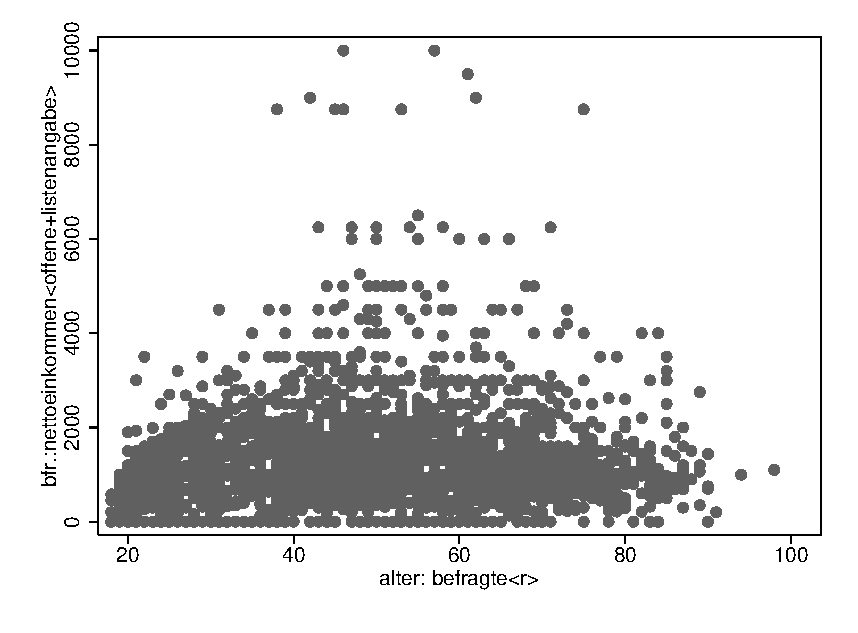
\includegraphics[width=8cm]{images/scatter.eps}}
\end{figure}
\end{frame}

\section{Boxplots}
\begin{frame}[fragile]{Boxplots} \index{Grafik!Boxplots} \index{Grafik!graph box}
\begin{lstlisting}
graph box hhinc
\end{lstlisting}
\begin{figure}
{\centering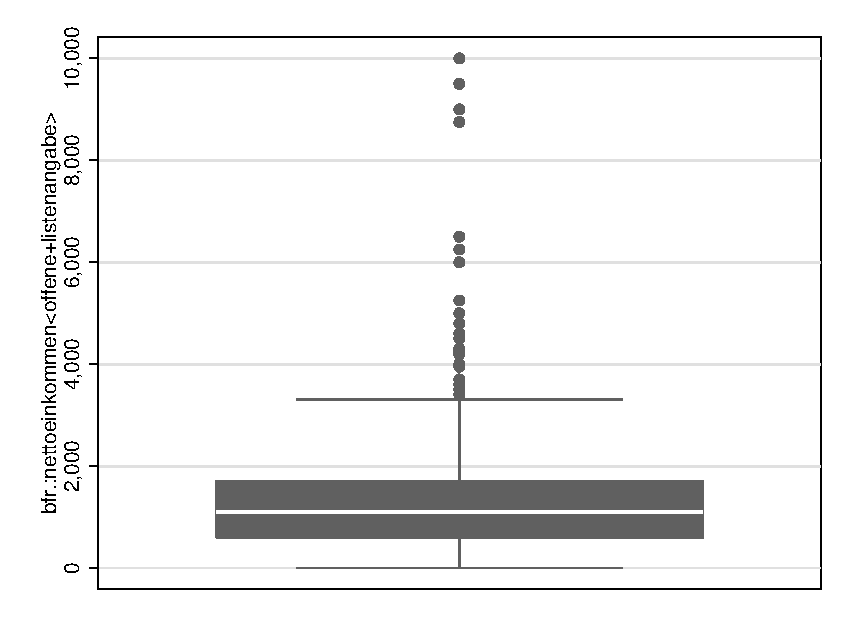
\includegraphics[width=8cm]{images/box.eps}}
\end{figure}
\end{frame}

\section{Histogramme}
\begin{frame}[fragile]{Histogramme} \index{Grafik!Histogramme} \index{Grafik!hist} \index{Grafik!hist freq}
\begin{lstlisting}
hist hhinc, freq
\end{lstlisting}
\begin{figure}
{\centering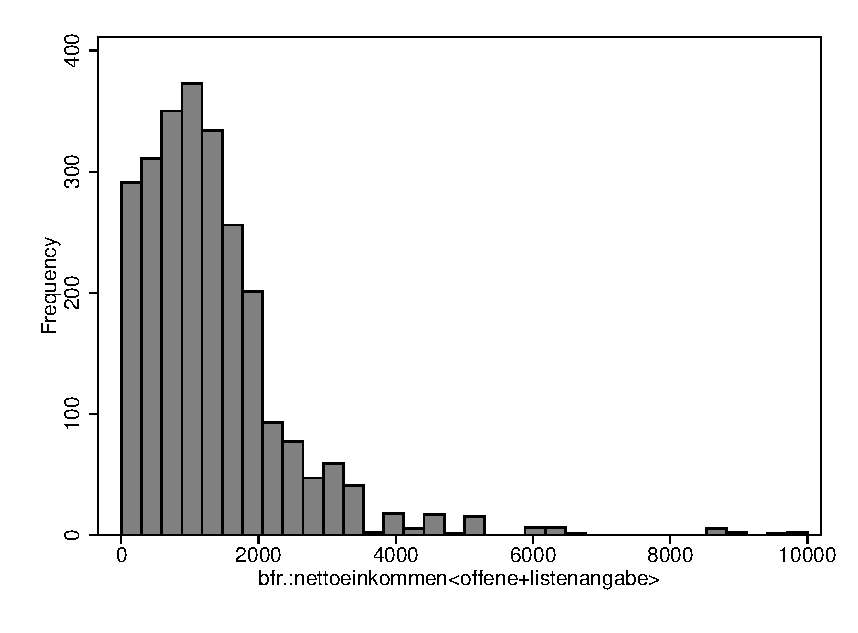
\includegraphics[width=8cm]{images/hist.eps}}
\end{figure}

  \begin{tikzpicture}[transform shape, rotate=10, overlay]
\node at (8,2) [mybox] (box) {%
    \begin{minipage}[t!]{0.35\textwidth}
    \tiny\textcolor{black}{\texttt{freq erzeugt Häufigkeiten, sonst steht auf der y-Achse die Dichte.}}
    \end{minipage}
    };
\end{tikzpicture}

\end{frame}

\section{Dot-Charts}
\begin{frame}[fragile]{Dot-Charts} \index{Grafik!Dot-Charts} \index{Grafik!graph dot} \index{Grafik! graph dot over()}
\begin{lstlisting}
graph dot (mean) hhinc, over(sex)
\end{lstlisting}
\begin{figure}
{\centering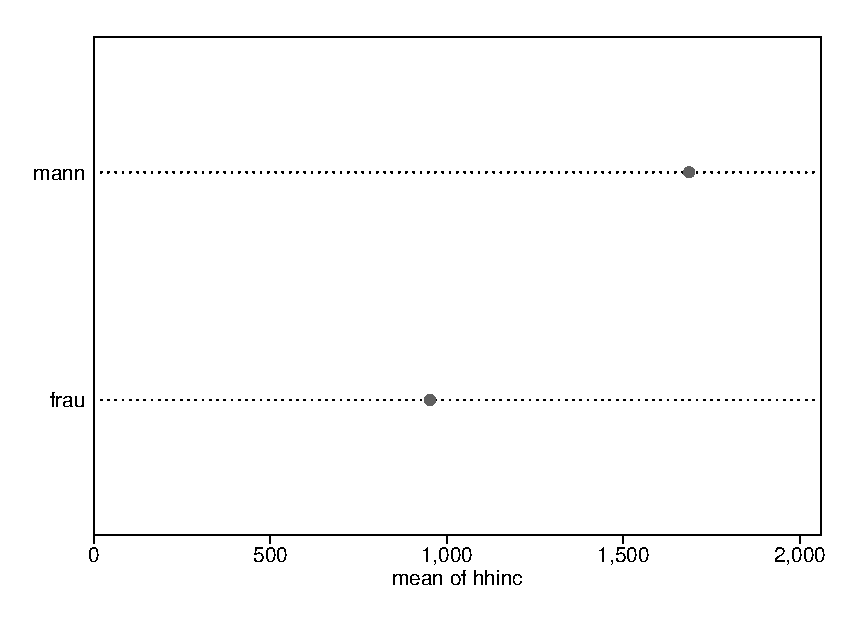
\includegraphics[width=8cm]{images/dot.eps}}
\end{figure}
\end{frame}


\section{Export von Grafiken}
\begin{frame}[fragile]{Export von Grafiken} \index{Grafik!exportieren}
\begin{lstlisting}
graph export "${OUTPUT}\graph1.pdf", replace
\end{lstlisting}
\begin{itemize}
\item Zum Export von Grafiken stehen mehrere Formate zur Verfügung
\item .ps .pes .wmf .emf .pdf .png .tif
\item Zur Weiterverarbeitung in MS-Office Programmen empfiehlt sich .png
\item Zur Weiterverarbeitung in TeX empfiehlt sich .pdf oder .eps
\end{itemize}
\end{frame}
%%%
%%% Improved Datahandling
%%%
\part{Improved Datahandling}
\begin{frame}
\thispagestyle{empty}
\textbf{\huge{Improved\\ Datahandling}}
\end{frame}

\begin{frame}{Improved\\ Datahandling Contents}
 \tableofcontents
\end{frame}

\section{by}
\begin{frame}[fragile]{by I} \index{by} \index{by!bysort}
Select subsets
\begin{lstlisting}
  summarize weight if sex == 1
  summarize weight if sex == 2
\end{lstlisting}

Do it in a single line
\begin{lstlisting}
  by edu, sort: summarize hhinc
\end{lstlisting}

  \begin{tikzpicture}[transform shape, rotate=10, overlay]
\node at (7.5,-0.5) [mybox] (box) {%
    \begin{minipage}[t!]{0.35\textwidth}
    \tiny\textcolor{black}{\texttt{by is not allowed with every command, in doubt contact the help. To use by cases have to be sorted. Alternativ: bysort}}
    \end{minipage}
    };
\end{tikzpicture}
\end{frame}

\begin{frame}[fragile]{by II}
It is possible to use more than one variable \index{by}
\begin{lstlisting}
  by sex county, sort: summarize weight
\end{lstlisting}
\end{frame}

\section{in}
\begin{frame}[fragile]{in}
Select only a few cases \index{list}
\begin{lstlisting}
  ** select the first
  list sex in 1
  ** select the first ten
  list sex in 1/10
\end{lstlisting}

  \begin{tikzpicture}[transform shape, rotate=10, overlay]
\node at (7.5,-0.5) [mybox] (box) {%
    \begin{minipage}[t!]{0.35\textwidth}
    \tiny\textcolor{black}{\texttt{Usually single cases are not interesting, but this can be helpful to spot strange cases.}}
    \end{minipage}
    };
\end{tikzpicture}
\end{frame}


\section{Loops}
\begin{frame}[fragile]{Loops I} \index{Loops} \index{Loops!foreach}
Loops in Stata. Example from \textcite[69f.]{Kohler2012}
\begin{lstlisting}
** Generate variables r1 - r10
** Newlist
foreach var of newlist r1-r10 {
  gen `var' = runiform()
}

** Numeric list
foreach num of numlist 1/10 {
  replace r`num' = runiform()
}
\end{lstlisting}
\end{frame}

\begin{frame}[fragile]{Loops II} \index{Loops} \index{Loops!foreach} \index{Loops!forvalues}
\begin{lstlisting}
** multiple commands in a loop
foreach var of varlist ybirth income {
  summarize `var', meanonly
  generate `var'_c = `var' - r(mean)
  label variable `var'_c "`var' (centered)"
}
\end{lstlisting}

\begin{lstlisting}
** Forvalues
forvalues num = 1/10 {
  replace r`num' = runiform()
}
\end{lstlisting}
\end{frame}

\section{log-files}
\begin{frame}[fragile]{log-files} \index{log} \index{log!log-files}
  \begin{itemize}
    \item Results can be stored in log-files.
    \item These contain all commands and their results.
    \item Logging begins after
    \begin{lstlisting}
  log using <dateiname.log>
    \end{lstlisting}
    \item log-files can be opened with every texteditor.
  \end{itemize}
\end{frame}

\begin{frame}[fragile]{log-files II}
  \begin{itemize} \index{log} \index{log!using} \index{log!close}
   \item Define a name and path where the log-file is saved. Usually the log-file name should reflect the do-files name.
   \begin{lstlisting}
  log using read-soep.log, replace
   \end{lstlisting}
   \item At the end of the do-file
   \begin{lstlisting}
  ** commands will not be logged after this
  log close
   \end{lstlisting}
   \item Thrown errors stop the do-files execution, therefore a manual closing of the log-file might be required because Stata cannot handle two open log-files
   \begin{lstlisting}
  log close
   \end{lstlisting}
  \end{itemize}
  
    \begin{tikzpicture}[transform shape, rotate=10, overlay]
\node at (7.5,-0.5) [mybox] (box) {%
    \begin{minipage}[t!]{0.35\textwidth}
    \tiny\textcolor{black}{\texttt{capture log close atop log using ensures that all open log-files will be closed.}}
    \end{minipage}
    };
\end{tikzpicture}
\end{frame}

\section{Macros}
\begin{frame}[fragile]{Macros} \index{Macros} \index{Macros!global}
With longer pathes and bigger projects it is helpful to use so called Macros. Macros may be global (it is known everywhere inside your code) or local (it is known only in a specific loop). We use macros for paths
\begin{lstlisting}
  ** global Macroname Pathname
  global DATA "D:/Data/data/original/"
  global OUT "D:/Data/data/bearbeitet/"
\end{lstlisting}
Now the macros can be called like this
\begin{lstlisting}
 cd "${DATA}"
\end{lstlisting}

\end{frame}

\begin{frame}[fragile]{Macros II}
It is especially helpfull handling long or different directorys for input, output, images or log files. Some additional examples \index{Macros}
\begin{lstlisting}
  use "${DATA}testdata.dta", clear
  save "${OUT}testdata_recoded.dta", replace
\end{lstlisting}
The syntax readability benefits a lot from this

  \begin{tikzpicture}[transform shape, rotate=10, overlay]
\node at (7.5,-2.1) [mybox] (box) {%
    \begin{minipage}[t!]{0.35\textwidth}
    \tiny\textcolor{black}{\texttt{You will save a lot of time. Long paths are written only once, which minimizes typos. A correct macro will be correct for the entire document. Still macros won't help you thinking.}}
    \end{minipage}
    };
\end{tikzpicture}

\end{frame}

\section{Using}
\begin{frame}[fragile]{using} \index{Import!use using} \index{Sort!sort}
Stata can handle only a limited range of variables, so a little housekeeping is advised.\footnote{Different Stata versions have different limits: IC (the version your working with) can handle $2,047$, SE can handle $32,767$ variables. Handling more variables is rather expensive. Prices for 2013: \$189 and \$395 for students. Non academic single user licenses \$$1545$ and \$$2090$.} Handling the SOEP this limit is not as far away as you might believe.
\begin{lstlisting}
  ** Import a minimal ppfad
  ** kepp only hhnr persnr sex gebjahr
  use hhnr persnr sex gebjahr using "${DATA}ppfad.dta"
  ** Sort cases by persnr and gebjahr
  sort persnr gebjahr
\end{lstlisting}
\end{frame}

\section{Merge}
\begin{frame}{merge} \index{Merge!merge}
\begin{minipage}{11cm}
In the Sozio-oekonomischen Panel (SOEP) (s. \cite{Wagner07}) each years data is split into different smaller data files. This has historical and maybe even practical reasons.\\
Starting from a file different of these data files share, we can combine the smaller files to generate a complete data set. This combination is called \textit{merging}.
\end{minipage}
\end{frame}

\begin{frame}[fragile]{merge II} \index{Merge!merge}
\begin{minipage}{11cm}
As example: We merge \textbf{ppfad} with \textbf{bep} and \textbf{bepgen}. ppfad is the key file for the person or p-context. \textbf{ppfad} is the data file every p-file shares. To make sure that we combine our data correctly for the p-context, we seek for matches in household-id (hhnr) and person-id (persnr).\\

\begin{tikzpicture}[thick]
\node at ( 3,2) [rectangle,draw=black,text width=4cm,align=center] (ppfad) {ppfad \\
									    hhnr, persnr};

\node at ( 0,0) [rectangle,draw=black,text width=4cm,align=center] (bekind) {bep \\
									    hhnr, persnr};
\node at ( 6,0) [rectangle,draw=black,text width=4cm,align=center] (bepgen) {bepgen \\
									    hhnr, persnr};
									    
\draw[->] (bekind) -- (ppfad);
\draw[->] (bepgen) -- (ppfad);
\end{tikzpicture}
\end{minipage}
\end{frame}


\begin{frame}[fragile]{merge III}
Running \texttt{merge} \index{Merge!merge}

\begin{lstlisting}
  ** merge ppfad with 2014 bep
  merge 1:1 persnr using "${DATA}bep.dta"
\end{lstlisting}

\begin{table}
\begin{center}
\begin{scriptsize}
\begin{tabular}{lll}
 Result & \# of obs. & \\ 
 \midrule
 not matched & 25,834 & \\
 ~~from master & 25,834  &(\_merge==1) \\
 ~~from using  & 0 &(\_merge==2) \\
 & & \\
 matched & 10,471 & (\_merge==3) \\
 \midrule
\end{tabular}
\end{scriptsize}
\end{center}
\end{table}
This means 
\begin{itemize}
 \item $25,834$ cases of \texttt{ppfad} were not found in \texttt{bep}.
 \item $0$ cases of \texttt{bep} were not found in \texttt{ppfad}
 \item $10,471$ cases of \texttt{bep} were found in \texttt{ppfad}
\end{itemize}
\end{frame}

\begin{frame}[fragile]{merge IV}\index{Merge!\_merge}\index{Merge!merge}
\begin{minipage}{11cm}
A new variable \texttt{\_merge} is created containing the \texttt{\_merge==} values. For now we remove all cases where we could not find a match from \texttt{using} which is \texttt{\_merge==2}. These are potentially problematic as we have no information about these persons sex or year of birth. Luckily at our current stage these are zero cases. Afterwards we remove \texttt{\_merge}.
\begin{lstlisting}
  ** Drop if using does not match master
  drop if _merge==2
  ** drop _merge
  drop _merge
\end{lstlisting}
\end{minipage}


  \begin{tikzpicture}[transform shape, rotate=10, overlay]
\node at (7.5,-1.5) [mybox] (box) {%
    \begin{minipage}[t!]{0.35\textwidth}
    \tiny\textcolor{black}{\texttt{The coice which merge is dropped is depending on the analysis.}}
    \end{minipage}
    };
\end{tikzpicture}

\end{frame}

\begin{frame}[fragile]{merge V} \index{Merge!merge} \index{Merge!merge, keepusing}
Example: merge with the generated variable highest educational achievement \texttt{bepsbil} from data-file \textbf{bepgen}.

\begin{lstlisting}
  merge 1:1 hhnr persnr using "${DATA}bepgen.dta", keepusing(bepsbil)
  drop if _merge==2
  drop _merge
\end{lstlisting}

  \begin{tikzpicture}[transform shape, rotate=10, overlay]
\node at (7.5,-1.5) [mybox] (box) {%
    \begin{minipage}[t!]{0.35\textwidth}
    \tiny\textcolor{black}{\texttt{\textbf{bepgen} contains $65$ variables, but all we need is the educational achievement.}}
    \end{minipage}
    };
\end{tikzpicture}
\end{frame}

\section{Operators}
\begin{frame}[fragile]{Operators} \index{Operators}
Stata lists the following operators, which can be used with variables. Using \texttt{var1\^{}2} every value of \texttt{var1} will be squared.
\begin{lstlisting}
 == // equals
 != // not equal ~=
 & // and
 | // or
 ! // not
 < // smaller
 > // greater
 <= // smaller equal
 >= // greater equal
 + // plus
 - // minus
 / // divide
 * // mutiply
 ^ // power
\end{lstlisting}
\end{frame}

\begin{frame}[fragile]{Functions} \index{Functions}
Additionaly Stata contains a range of built in functions (\texttt{help functions}).
A selection:
\begin{lstlisting}
  abs() // absolute value/modulus |-2| == 2
  max() // greates value
  min() // smalles value
  exp() // e-function
  ln() // logarithm
  round() // round
  sin() // Sinus
  sqrt() // square root
  runiform() // random number
\end{lstlisting}
\end{frame}
%%%
%%% Statistik
%%%
\part{Statistik}
\begin{frame}
\thispagestyle{empty}
\textbf{\huge{Statistik}}
\end{frame}

\begin{frame}{Statistik Inhalt}
 \tableofcontents
\end{frame}


\section{Maßzahlen}
\begin{frame}[fragile]{Maßzahlen I}
Arithmetisches Mittel und ein paar Maßzahlen \index{Mittelwert!mean} \index{Beschreiben!summarize} \index{Beschreiben!detail} \index{Mittelwert} \index{Maßzahlen}
\begin{lstlisting}
  mean sex
  summarize sex
  summarize sex, detail
\end{lstlisting}

  \begin{tikzpicture}[transform shape, rotate=10, overlay]
\node at (8,-1.5) [mybox] (box) {%
    \begin{minipage}[t!]{0.35\textwidth}
    \tiny\textcolor{black}{\texttt{mean gibt den Standardfehler aus: $s/\sqrt{n}$. summarize gibt die Standardabweichung aus: $\sqrt{\sum(x-\bar{x})^2)/n}$.}}
    \end{minipage}
    };
\end{tikzpicture}
\end{frame}


\begin{frame}[fragile]{Maßzahlen II}
Minimum, Maximum, arithmetisches Mittel, Median, Anzahl und Quartile. \index{Minimum} \index{Minimum!min} \index{Maximum} \index{Maximum!max} \index{Mittelwert!mean} \index{Mittelwert} \index{Mittelwert!Arithmetisches Mittel} \index{Mittelwert!Median} \index{Quantile} \index{tabstat} \index{Range} \index{Range!range} \index{Quantile!q}
\begin{lstlisting}
  tabstat age, statistic(min max mean median p50)
  tabstat age, statistic(min max range mean count q) by(sex)
\end{lstlisting}

  \begin{tikzpicture}[transform shape, rotate=10, overlay]
\node at (8,-1.5) [mybox] (box) {%
    \begin{minipage}[t!]{0.35\textwidth}
    \tiny\textcolor{black}{\texttt{range = max - min}}
    \end{minipage}
    };
\end{tikzpicture}
\end{frame}


\begin{frame}[fragile]{Maßzahlen III}
Standardabweichung, Standardfehler, Varianz und Interquartilsabstand. \index{Standardabweichung} \index{Standardfehler} \index{Varianz} \index{Interquartilsabstand} \index{tabstat} \index{Standardabweichung!sd} \index{Varianz!var} \index{Standardfehler!sem} \index{Interquartilsabstand!iqr} \index{Quantile!q} \index{Schiefe} \index{Wölbung} \index{Schiefe!skewness} \index{Wölbung!kurtosis}
\begin{lstlisting}
 tabstat age, statistic(sd sem var q iqr)
\end{lstlisting}
Schiefe und Wölbung
\begin{lstlisting}
  tabstat age, statistics(skewness kurtosis)
\end{lstlisting}

  \begin{tikzpicture}[transform shape, rotate=10, overlay]
\node at (8,-1.5) [mybox] (box) {%
    \begin{minipage}[t!]{0.35\textwidth}
    \tiny\textcolor{black}{\texttt{iqr = q3 - q1}}
    \end{minipage}
    };
\end{tikzpicture}
\end{frame}

\section{Tabellen}
\begin{frame}[fragile]{Tabellen} \index{Tabelle!tab} \index{Tabelle!tab, summarize()} \index{Tabelle}
Wir hatten bereits \texttt{summarize} und \texttt{tab}, jetzt kombinieren wir
\begin{lstlisting}
  tab sex, summarize(age)
\end{lstlisting}
\end{frame}

\subsection{Kreuztabellen}
\begin{frame}[fragile]{Kreuztabellen} \index{Tabelle!tab} \index{Tabelle!tab1} \index{Tabelle!tab2} \index{Tabelle!Kreuztabelle}
Kreuztabellen erzeugen mit
\begin{lstlisting}
  tab sex east
\end{lstlisting}
Weitere Tabellen
\begin{lstlisting}
  ** Tabellen von jeder der drei Variablen
  tab1 sex age edu
  ** Kreuztabellen ab bc ac
  tab2 sex age edu
\end{lstlisting}
\end{frame}

\subsection{Chi, V und Phi}
\begin{frame}[fragile]{Kreuztabellen II} \index{Tabelle!Kreuztabelle} \index{Tabelle!$\chi^2$} \index{Tabelle!chi-square} \index{Tabelle!chi} \index{Tabelle!tab} \index{Tabelle!Cramers V} \index{Tabelle!tab exp} \index{Tabelle!tab col} \index{Tabelle!tab row}
Die Statistik I Vorlesung rekapitulieren, wir machen ein paar Tests \footnote{Oder nachschlagen z.~B. bei \textcite{Krebs10} oder \textcite{Agresti09}. }
\begin{lstlisting}
  ** chi-quadrat
  tab sex east, chi
  ** cramers v
  tab sex east, V
  ** wer per Hand nachrechnen will
  tab sex east, exp col row
  ** phi manuell ausrechnen
  di (934*426-441*1026) / (1375*1452*1960*867)^(1/2)
  di 2827 *(-.02963311)^2 // == chi^2
\end{lstlisting}

\end{frame}

\begin{frame}[fragile]{Numlabel}
Falls man die numerischen Werte auch im Label haben möchte \index{Label!numlabel}
\begin{lstlisting}
  ** numerische Label an für alle Variablen
  numlabel _all, add
  ** numerische Label aus
  numlabel _all, remove
\end{lstlisting}

\end{frame}

\section{Inferenz}
\begin{frame}[fragile]{T-Test} \index{T-Test!ttest} \index{T-Test}
Teststatistik
\begin{lstlisting}
  ** Vergleich Männer Frauen in West Ost
  tab sex, sum(east)
  ttest sex, by(east)
\end{lstlisting}
\end{frame}

\begin{frame}[fragile]{Und noch viel mehr \dots} \index{Regression!regress} \index{Regression!logit} \index{Regression!mlog}
Regression
\begin{lstlisting}
  regress
  logit
  mlog
\end{lstlisting}
\end{frame}

\begin{frame}
\thispagestyle{empty}
 Fortsetzung folgt.
\end{frame}



\part{Index und Literatur}
\begin{frame}
\thispagestyle{empty}
\textbf{\huge{Index \\ and Literature}}
\end{frame}

\section{Index}
\begin{frame}{Index}
\setlength{\columnseprule}{.4pt} 
\begin{multicols}{5}
 \begin{miniscule}
\printindex
 \end{miniscule}
\end{multicols}
\end{frame}

\section{Literature}
\begin{frame}[allowframebreaks]{Literature}
 \printbibliography[title=none]
\end{frame}

\end{document}
